\documentclass[12pt,oneside]{book}
%------------------------------------------------
% Font/Symbol Options
%------------------------------------------------
\usepackage{mathptmx} % sets times fronts and mathsymbols
\usepackage{amssymb} % additional symbols not in mathptmx
\usepackage{mathtools} % package for improving math fonts
\usepackage[T1]{fontenc} % allows the use of glpys and special characters
\usepackage{relsize} % package for changing font size
\usepackage{xcolor} % foreground and background color management
\usepackage{soul} % package for hyphens, underlines, strike out, etc
\usepackage{enumerate} % allows numbered lists building on itemize
\usepackage{upquote} % sets quote style
\usepackage{moreverb} % allows the use of verbatim
\usepackage{gensymb} % provides gen symbols for math like \degree
\usepackage{ragged2e} % helps space words and hyphenate word wrap
\usepackage[titles]{tocloft} % control over the typography of the Table of Contents, List of Figures and List of Tables

% Colors used for cross references and table colors
\definecolor{linknavy}{rgb}{0,0,0.50196}
\definecolor{linkred}{rgb}{1,0,0}
\definecolor{linkblue}{rgb}{0,0,1}

%------------------------------------------------
% Float Options
%------------------------------------------------
\usepackage[pdftex]{graphicx} % improves includegraphics
\usepackage{caption} % customise the captions in floating environments like figure and table
\usepackage{subcaption}
\usepackage{xltabular} % keeps tabularx which helps with column management and but adds longtable
\newcolumntype{L}[1]{>{\raggedright\let\newline\\\arraybackslash\hspace{0pt}}m{#1}}
\newcolumntype{C}[1]{>{\centering\let\newline\\\arraybackslash\hspace{0pt}}m{#1}}
\newcolumntype{R}[1]{>{\raggedleft\let\newline\\\arraybackslash\hspace{0pt}}m{#1}}
\usepackage{booktabs} % high quality tables - allows toprule, midrule, etc
\usepackage{array} % extended implementation of the array and tabular environments which extends the options for column formats
\usepackage{float} % Improves the interface for defining floating objects such as figures and tables
\usepackage{placeins} % provides use of FloatBarrier for managing floats
% \usepackage{subfig} % provides ability to use subfigures
\usepackage{threeparttable} % allows for tablenotes
\usepackage{multirow} % allows split rows

% \usepackage{colortbl} % allows rows and cols of tables to be colored
% \definecolor{lbcolor}{rgb}{0.96,0.96,0.96}

%------------------------------------------------
% Crossref and Bibliography Options
%------------------------------------------------
\newcommand{\nopart}{\expandafter\def\csname Parent-1\endcsname{}} % To fix table of contents in pdf.

\usepackage{cite} %bibliography management
\usepackage{notoccite} % prevents references counting in figures/TOCs superceeding true numbering
\newcommand\notype[1]{\unskip} % allows skip of type for citing research reports
\usepackage[nottoc,notlof,notlot]{tocbibind} % Put the bibliography and index in the ToC
\usepackage[toc,page]{appendix} %defines appendix

%------------------------------------------------
% Output and Page Options
%------------------------------------------------

\renewcommand{\chaptername}{} % drops the word chapter
\renewcommand{\bibname}{References} % renames bibliography to references

\usepackage[pdftex,
        colorlinks=true,
        urlcolor=linkblue,     % \href{...}{...} external (URL)
        citecolor=linkred,     % citation number colors
        linkcolor=linknavy,    % \ref{...} and \pageref{...}
        pdfproducer={pdflatex},
        pdfpagemode=UseNone,
        bookmarksopen=true,
        plainpages=false,
        verbose]{hyperref} %handles cross references

\usepackage{geometry} % user interface to customize page layout

\setlength{\textwidth}{6.5in}
\setlength{\textheight}{9.0in}
\setlength{\topmargin}{0.in}
\setlength{\headheight}{0.pt}
\setlength{\headsep}{0.in}
\setlength{\parindent}{0.0in}
\setlength{\itemindent}{0.25in}
\setlength{\oddsidemargin}{0.0in}
\setlength{\evensidemargin}{0.0in}
% \setlength{\leftmargini}{\parindent} % Controls the indenting of the "bullets" in a list
\setlength{\cftsecnumwidth}{0.45in}
\setlength{\cftsubsecnumwidth}{0.5in}
\setlength{\cftfignumwidth}{0.45in}
\setlength{\cfttabnumwidth}{0.45in}
\setlength{\parskip}{1em}

\usepackage{fancyhdr}
\pagestyle{fancy}
\lhead{}
\rhead{}
\chead{}
\renewcommand{\headrulewidth}{0pt}

\usepackage{titlesec} % sets title stying
\titleformat{\chapter}[hang]{\normalfont\huge\bfseries}{\chaptertitlename\thechapter}{1em}{}
\titlespacing*{\chapter}{0pt}{-30pt}{20pt}

%------------------------------------------------
% Misc Optional Packages
%------------------------------------------------
\usepackage{setspace}
\usepackage{scrextend}
% \usepackage{calc} % simple arithmetic commands -- \setcounter,\setlength
% \usepackage{makeidx} % Create index at end of document
% \usepackage{lastpage} % Automatic last page number reference.
% \usepackage{xfrac} % Improves quality of fractions inline mathmode and in equations
% \usepackage{paralist} % inline lists
% \usepackage{varwidth} % variable width minipage
% \usepackage{listings} % allows user to typeset code inline
% \usepackage{tikz} % drawing package
\usepackage[version=4]{mhchem} % typesetting chemical molecular formulae and equations
% \usepackage{rotating} % rotated boxes (or floats, which are themselves boxes), and boxes always stay on one page.
% \usepackage{lscape} % continuous text (i.e., more than one page) set in landscape mode
% \usepackage{longtable} % allows tables to flow across pages

\usepackage{siunitx} %typsetting units
\sisetup{
    detect-all = true,
    input-decimal-markers = {.},
    input-ignore = {,},
    inter-unit-product = \ensuremath{{}\cdot{}},
    multi-part-units = repeat,
    number-unit-product = \text{~},
    per-mode = fraction,
    separate-uncertainty = true,
}

% \floatstyle{boxed}
% \newfloat{notebox}{H}{lon}
% \newfloat{warning}{H}{low}

% \newenvironment{conditions}
%   {\par\vspace{\abovedisplayskip}\noindent\begin{tabular}{>{$}l<{$} @{${}={}$} l}}
%   {\end{tabular}\par\vspace{\belowdisplayskip}}

%------------------------------------------------
% Title page definitions
%------------------------------------------------

\newcommand{\titlesigs}{\medskip
	\large \flushleft{UL Research Institutes} \\
	{Terrence R. Brady, President} \\
	{Christopher J. Cramer, Chief Research Officer} \\ \medskip
	\flushleft{Fire Safety Research Institute \\
		{Steve Kerber, Vice President and Executive Director} \\
		\hspace{1in} \\}}


\newcommand{\titleA}{\flushleft{\huge\bf{\vartitle}}}
\newcommand{\titleB}{\vspace{.5in}\flushleft{\large\flushleft{\varauthors\vspace{0.2in}\varaddress\vspace{0.2in}\vardate}}}
\newcommand{\titleC}{\vspace{.3in}\flushleft{\large\flushleft{This publication is available free of charge from:\\ \vardoi}}}
\newcommand{\titleD}{
	\begin{minipage}{0.35\textwidth}
		\begin{flushleft}
			
\includegraphics[width=1\textwidth]{../Bibliography/UL_RI}
		\end{flushleft}
	\end{minipage}
	\hfill
	\begin{minipage}{0.5\textwidth}
		\begin{flushright}
			
\includegraphics[width=1.25in]{../Bibliography/FSRI_Logo_white}
		\end{flushright}
	\end{minipage}
}
\newcommand{\titleE}{\scriptsize\flushleft{\textcopyright \the\year{}. UL Research Institutes. All rights reserved.}}


\newcommand{\forceindent}{\leavevmode{\parindent=1em\indent}}
% -----------------------------------------------
% Set Report Title and Authors
% -----------------------------------------------
\newcommand{\vartitle}{Materials and Products Database - User Guide\\}
\newcommand{\vardate}{\today \\}
\newcommand{\varauthors}{Mark McKinnon \\
						Craig Weinschenk \\}
\newcommand{\varaddress}{Fire Safety Research Institute \\
	UL Research Institutes\\
	Columbia, MD 21045 \\}
\newcommand{\vardoi}{\url{https://dx.doi.org/10.54206/XXXXXXXX}}


\begin{document}
\pagenumbering{gobble}
\bibliographystyle{unsrturl}
\urlstyle{rm}
\hypersetup{pageanchor=false}

% Custom Commands
\newcommand*\degC[1]{{#1}~\textdegree C}  % \degC{22}

%------------------------------------------------
% Title Page 1
%------------------------------------------------
\begin{minipage}[t][9in][s]{6.25in}
\titleA
\titleB
\titleC
\vfill
\titleD
\titleE
\end{minipage}

%------------------------------------------------
% Blank page between Title Pages
%------------------------------------------------

\newpage
\hspace{5in}
\newpage

%------------------------------------------------
% Title Page 3
%------------------------------------------------

\begin{minipage}[t][9in][s]{6.25in}
\pagenumbering{gobble}
\titleA
\titleB
\titleC
\vfill
\titlesigs
\titleD
\titleE
\end{minipage}
\newpage

\begin{minipage}[t][9in][s]{6.25in}

\flushleft{In no event shall UL Research Institutes be responsible to anyone for whatever use or non-use is made of the information contained in this Report and in no event shall UL Research Institutes, its employees, or its agents incur any obligation or liability for damages including, but not limited to, consequential damage arising out of or in connection  with the use or inability to use the information contained in this Report. Information conveyed by this Report applies only to the specimens actually involved in these tests. UL Research Institutes has not established a factory Follow-Up Service Program to determine the conformance of subsequently produced material, nor has any provision been made to apply any registered mark of UL to such material. The issuance of this Report in no way implies Listing, Classification or Recognition by UL Enterprises and does not authorize the use of UL Listing, Classification or Recognition Marks or other reference to UL Enterprises on or in connection with the product or system.
}

\vspace{3in}
\vfill
\hspace{1in}

\end{minipage}

\newpage

\hypersetup{pageanchor=true}

\newpage
\frontmatter

\pagestyle{plain}
\pagenumbering{roman}

\cleardoublepage
\phantomsection
\tableofcontents

\cleardoublepage
\phantomsection
\addcontentsline{toc}{chapter}{List of Figures}
\listoffigures

% \cleardoublepage
% \phantomsection
% \addcontentsline{toc}{chapter}{List of Tables}
% \listoftables

\chapter*{\centering Acknowledgments}

\begin{table}[!ht]
	\centering
	\caption*{Project Technical Panel}
	\begin{tabular}{ll}
		\toprule[1.5pt]
		Name & Affiliation \\ 
		\midrule
		Vyto Babrauskas	 	& Fire Science and Technology Inc \\
		Ernest Barile	 	& Philadelphia Fire Department \\
		Nicole Brewer	 	& Portland Fire \& Rescue \\
		Morgan Bruns	 	& St. Mary's University of Texas \\		
		Steve Carman 		& Carman \& Associates Fire Investigation, Inc \\
		Paul Claflin 		& Bureau of ATF, Fire Investigation \& Arson Enforcement Division \\
		Jason Dress	    	& Bureau of ATF, Fire Research Laboratory \\
		Adam Friedman	    & Bureau of ATF, Fire Research Laboratory\\
		Brian Geraci 		& Maryland State Fire Marshal \\
		Barry Grimm 		& International Association of Arson Investigators \\
		Brian Lattimer	 	& Virginia Polytechnic Institute and State University \\
		Chris Lautenberger	& Reax Engineering \\
		Kevin McGrattan 	& National Institute of Standards and Technology \\ 
		Tom Sabella 		& Fire Department City of New York, Retired \\
		Stanislav Stoliarov	& University of Maryland \\ 
		\bottomrule[1.25pt]
	\end{tabular}
\end{table}

\chapter*{List of Abbreviations}

\begin{tabbing}
\hspace{1.5in} \= \\
DSC 	\> Differential scanning calorimetry \\
FSRI    \> Fire Safety Research Institute \\
FTIR 	\> Fourier transform infrared spectrometer \\
HFM 	\> Heat flow meter \\
IS 		\> Integrating sphere \\
MCC 	\> Microscale combustion calorimetry \\
NIJ 	\> National Institute of Justice \\
NIST    \> National Institute of Standards and Technology \\
STA 	\> Simultaneous thermal analyzer \\
TGA 	\> Thermogravimetric analysis \\
\end{tabbing}

\newpage

\pagenumbering{arabic}
\setcounter{page}{1}

\newpage
\mainmatter
\newpage

\chapter{Introduction}
\label{sec:introduction}

For the past several years, the NIJ Technology Working Group's Operational Requirements for Fire and Arson Investigation have included several scientific research needs that require improved knowledge of properties of materials that are common in the built environment, and therefore likely to be involved in a fire scene. The specific areas of research include: adequate materials data inputs for accurate computer models, understanding the effect of materials properties on the development and interpretation of fire patterns, and evaluation of incident heat flux profiles to walls and neighboring items in support of fire model validation. Each of the three aforementioned research topics rely, in part, on accurate knowledge of the physical conditions of a material prior to the fire, how the material will respond to the exposure of heat, and how it will perform once it has ignited. The project described herein has made advancements in terms of collecting experimental data and property information on a multitude of materials commonly encountered in the built environment for the purpose of making the data publicly available and easily accessible to fire investigators, fire protection engineers, and fire researchers.

The database described in this document, Materials and Products Database, is an interactive, web-based repository populated with data from rigorous testing of the contemporary products and materials commonly found in the modern built environment -- \href{https://materials.fsri.org}{Materials and Products Database}. The backend of the database is open-access via public Github repository -- \href{https://github.com/ulfsri/fsri_materials_database}{fsri\_materials\_database}. The goal of this document is to provide information regarding the structure of the repository and corresponding front end website.

\chapter{Github Repository}
\label{sec:repo}

The public Github repository can be accessed here: \href{https://github.com/ulfsri/fsri_materials_database}{fsri\_materials\_database}. The repository contains the experimental data ({\bf 01\_Data}) and analysis scripts ({\bf 02\_Scripts}) for all of the materials tested. 

\section{Experimental Data}

Raw data generated from each apparatus are included in their respective folders for each material in plain-text format. Figure~\ref{fig:mat_list} is a partial list of the materials in the repository as displayed in Github.

\begin{figure}[!ht]
\centering
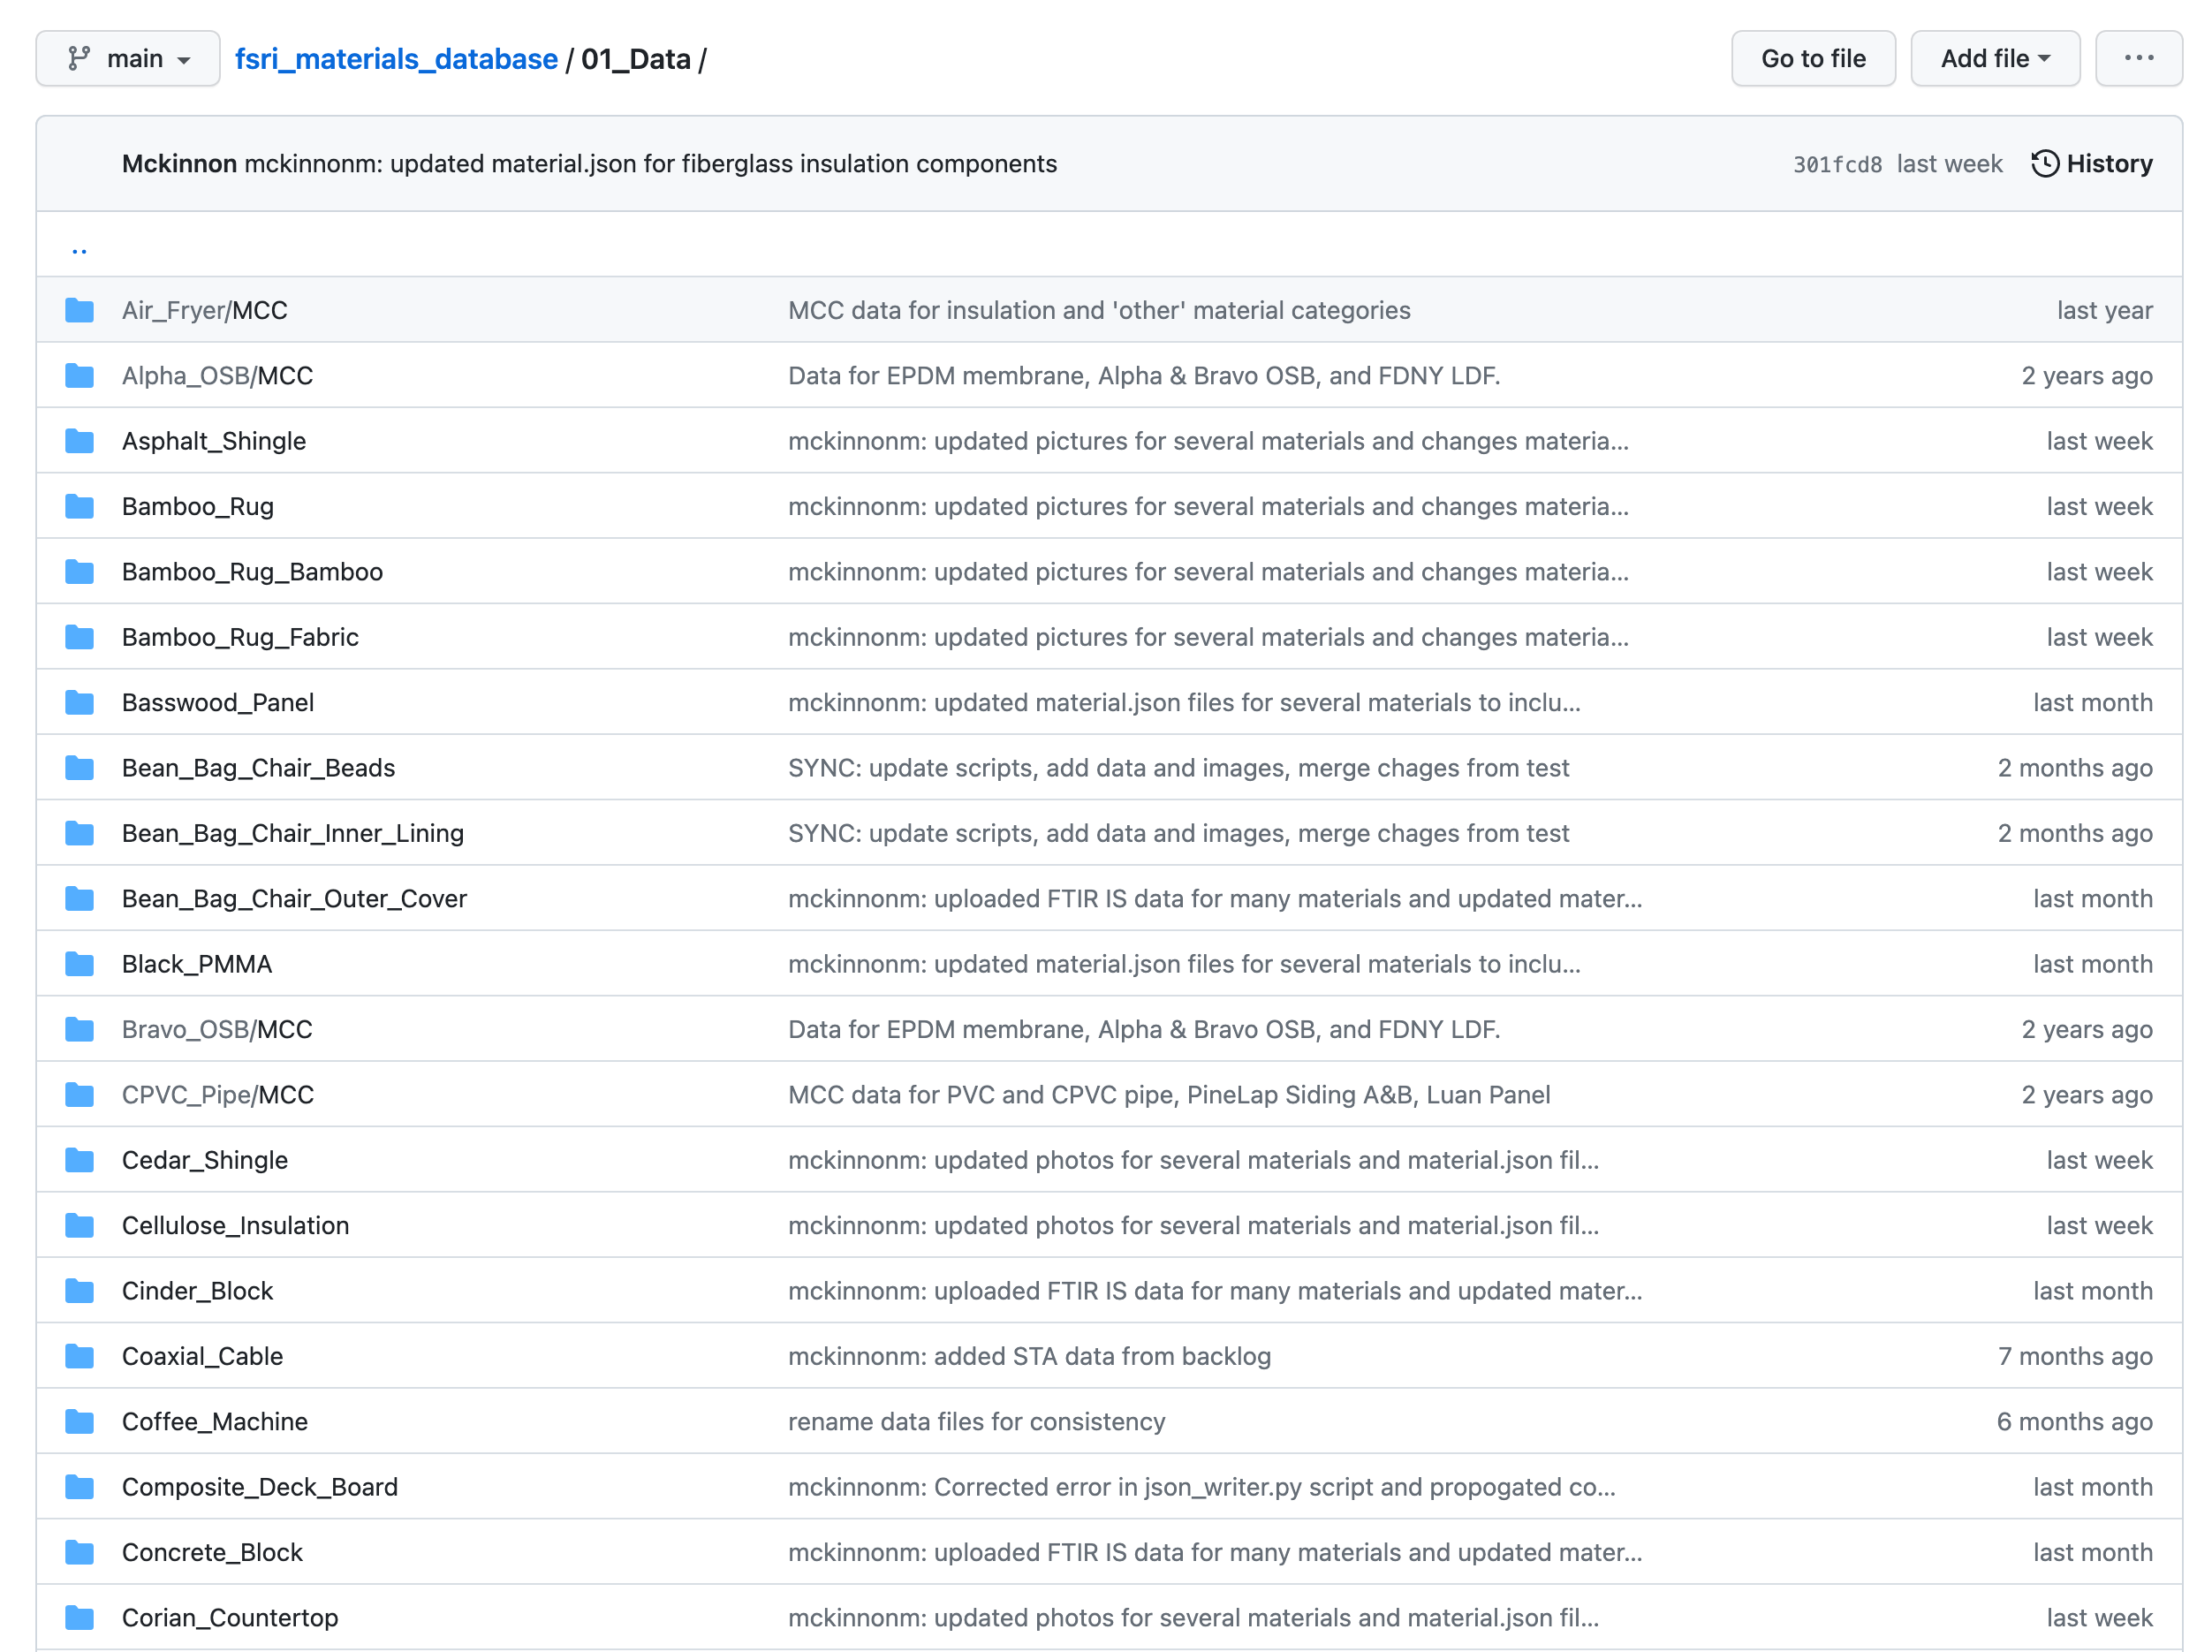
\includegraphics[width=.95\columnwidth]{Figures/partial_materials_github}
\caption[Partial List of Materials from Github Repository]{Partial list of materials from {\bf 01\_Data} in the \href{https://github.com/ulfsri/fsri_materials_database}{fsri\_materials\_database} Github repository.}
\label{fig:mat_list}
\end{figure}

Within each material directory, the data is organized by the short name of test apparatus used (e.g, Cone, HFM, etc.) and where applicable additional filtering by test settings (e.g., 3K\_min, 10\_min for the STA). An example of a material directory is included in Figure~\ref{fig:mat_example}. The following sections describe the data organization for each of the test apparatus used to generate the data.

\begin{figure}[!ht]
\centering
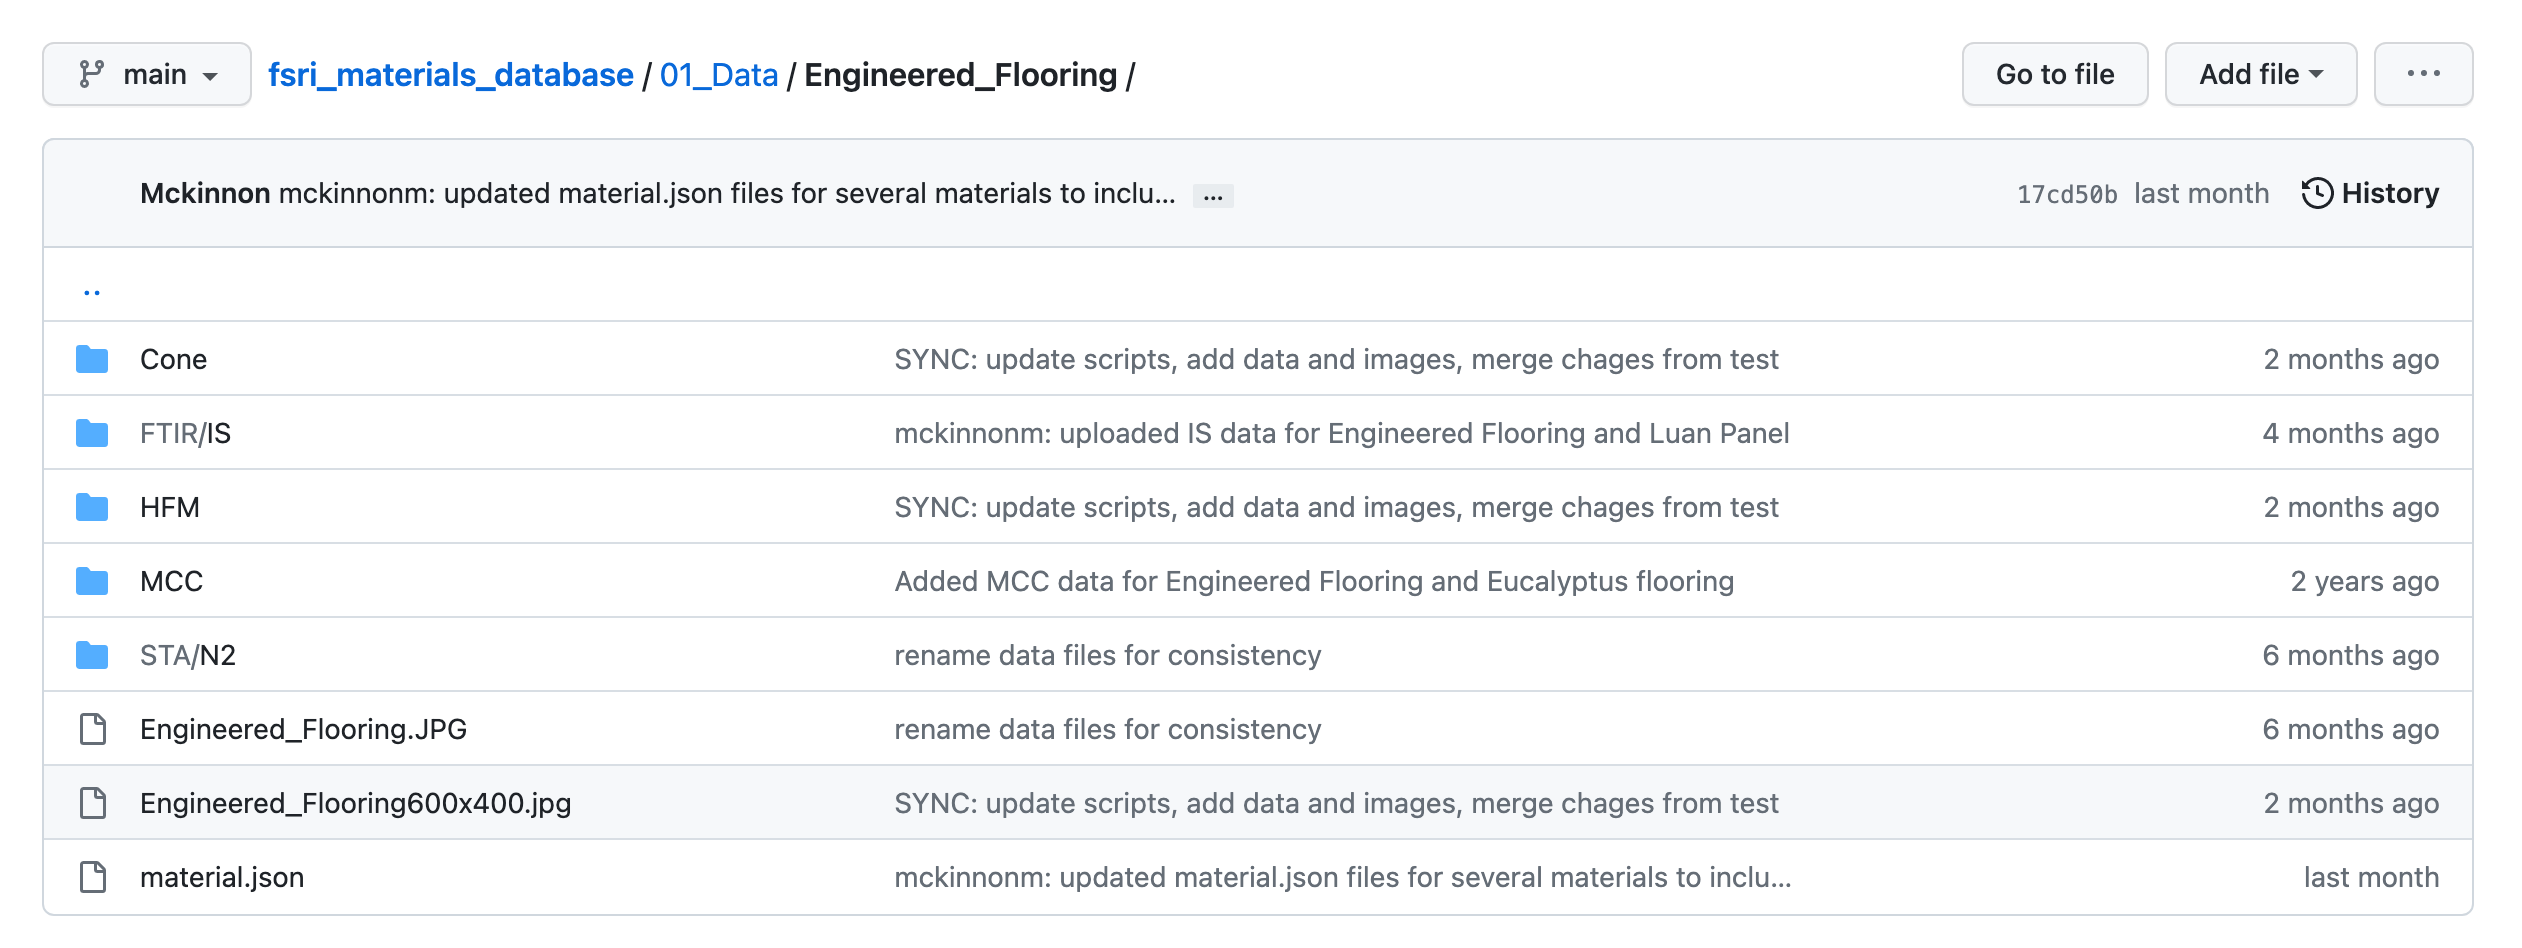
\includegraphics[width=.95\columnwidth]{Figures/engineered_flooring_example}
\caption[Engineered Flooring Material Directory Example]{Example directory structure from engineered flooring.}
\label{fig:mat_example}
\end{figure}

\subsection{material.json}
Each material that is included on the website has a material.json file. The file contains the text description of the material, where the material was procured from, material density, the length scale at which the material was tested (milligram, bench scale, full scale, large scale), and the applicable material category or categories. Materials fit into at least one of eleven categories: cord and cable, engineered wood, exterior finish, general polymer, insulation, interior finish, plumbing,roofing,sleeping product,structural, upholstered furniture. To broaden search capabilities, alternate names for materials (e.g., trade names, common names, etc.) are also included in the json file.

The core function of each json file is to link the graphs and tables produced by the included *\_html.py scripts to the respective landing page for each material on the website. At the top level of the repository exists {\em global.json} file. This file sets the overall structure of how the data is linked between the Github repository and the  website. The global json file establishes each of the measured and derived quantities that can appear on the website. Within each property a high level description of the tests are included as well as flags that set whether the a table, graph, or both are included. At the local material level, the test description can be overwritten if the experiments for the specific material deviated from baseline. Based on the graph/table flags set at the global level, the material file points to file path for required graphs and tables for the respective quantities. Note, only those quantities defined in the material file appear on the website. Further, materials in the repository that do not have a material.json file, will not appear on the website.

\subsection{Cone Calorimeter (Cone)}
The data file structure includes the material, the short name for the apparatus (cone), heat flux setting, scan/scalar, date of test, and replicate number. Scan is for the raw output data and scalar is for the initial conditions and high-level test parameters. For materials whose experiments deviated from typical behavior relevant pictures are included in the respective material directory. Any anomaly behaviors are included in the post test comment in the scalar data. This information is aggregated into a cone notes file that is produced by the {\em plot\_Cone\_data.py} script.

{\bf Data File Example:} MDF\_Cone\_HF25scalar\_210323\_R1 stands for the first replicate of scalar data generated from a medium density fiber board test in cone calorimeter exposed to 25 kW/m$^2$ on March 23, 2021.

\subsection{Fourier Transform Infrared Spectrometer (FTIR)}
The FTIR directory contains subdirectories for the Attenuated Total Reflectance method (ATR) and the Integrating Sphere (IS). Data file structure for the ATR experiment files includes the material, the abbreviated name for the apparatus, date of test, and replicate number.

{\bf Data File Example:} MDF\_ATR\_210323\_R5 stands for the fifth replicate of data collected with the ATR accessory conducted on June 8, 2021.

Data file structure for the IS experiment files includes the material, the abbreviated name for the apparatus, the measurand, whether the test is a sample measurement or standard reference, date of test, and replicate number.

{\bf Data File Example:} OSB\_IS\_REFLECT\_MEAS\_210623\_R2 stands for the second replicate conducted on oriented strand board to measure spectral reflection in the integrating sphere on June 23, 2021.

\subsection{Heat Flow Meter (HFM)}
Data file structure is the material, the abbreviated name for the apparatus, whether test was dry or wet, whether test was for thermal conductivity or heat capacity, date of test, and replicate number. Scan is for the raw output data and scalar is for the initial conditions and high-level test parameters.

{\bf Date File Example:} OSB\_HFM\_Dry\_Conductivity\_210315\_R3.tst stands for the third replicate of the data generated from an oriented strand board test in the heat flow meter tested dry for thermal conductivity on March 15, 2021.

\subsection{Micro-scale Combustion Calorimeter (MCC)}
Data file structure is the material, the abbreviated name for the apparatus, the heating rate in Kelvin per minute, date of test, and replicate number. Additionally, the final mass of the sample after the test is included in a separate text file named with the appendix 'FINAL\_MASS'.

{\bf Data File Example:} Polyester\_Fabric\_MCC\_30K\_min\_210308\_R1.csv stands for the first replicate of the data generated from a test on polyester fabric in the micro-scale combustion calorimeter tested with a heating rate of 30 Kelvin per minute on March 8, 2021.

\subsection{Simultaneous Thermal Analyzer (STA)}
Data file structure is the material, the abbreviated name for the apparatus, the atmosphere tested in, the heating rate in Kelvin per minute and data/meta, date of test, and replicate number. Data is for the raw output data and meta is for the initial conditions and high-level test parameters.

{\bf Data File Example:} Polyester\_Batting\_STA\_N2\_3KData\_210215\_R1.csv stands for the first replicate of the data generated from a polyester batting board test in the simultaneous thermal analyzer tested in nitrogen with a heating rate of 3 Kelvin per minute on March 15, 2021.

\subsection{Photos}
A full-size and thumbnail (600 x 400) photo are included for visualization on website. When applicable, additional photos are included to help describe anomalies that occurred during testing, in particular from cone calorimeter experiments.

\section{Processing Scripts}
\label{sec:scripts}

Python processing scripts exist for analyzing the experimental data to generate output quantities and to plot the experimental data. The scripts are apparatus specific and cycle through all materials upon execution. Each apparatus has a pair of scripts: data.py and data\_html.py.

To successfully execute the Python scripts in this repository, several additional packages (outside of base Python) will need to be installed. One way to do this is through pip with following commands:

\begin{verbatim}
pip install pandas              #used for data wrangling/processing
pip install numpy               #used for math analysis
pip install scipy               #used for stats analysis
pip install matplotlib          #used for plot styling and pdf plots
pip install plotly              #used for interactive html plots
pip install GitPython           #used for add repo hash to plots
pip install pybaselines         #used for melting analysis in STA
\end{verbatim}

The data.py script computes output quantities, produces reduced data .csv files, and produces .pdf graphs in 03\_Charts/Material/Apparatus. The output quantities and/or reduced data files are created in 01\_Data/Material/Apparatus. These files get updated each time the script gets executed.

The data\_html.py script produces interactive html files that allow interactions such as hover, zoom, and pan and html tables of relevant processed data. Similar to the data.py script, html graphs are output to 03\_Charts/Material/Apparatus and can be opened in a web browser.

To batch execute the scripts, run\_all.bat and run\_all.sh files exist for both the set of data.py scripts and the data\_html.py scripts. These files will execute the respective python scripts for each apparatus for all data in the repository.

If there are issues executing any script, in particular the .sh script, a change mode may be needed. In a command prompt type: chmod +x run\_all\_data.sh OR chmod +x run\_all\_data\_html.sh

When the scripts, either data.py or data\_html.py, are run, the current version of the repository (i.e., Github hash) is appended to the figure.

\subsection{Utilities}
This sub-directory contains scripts used to the build and manage the repository with a primary focus around generating the material.json files and maintaining package consistency.

\subsection{Deprecated}
This sub-directory contains legacy scripts that were used in prior analysis approaches. Although not the current approach used in the database, these scripts are included for as they may provide value to researchers looking to test different methodologies for processing the experimental data.


\section{Graphs and Tables}
\label{sec:graphs}

None of the graphs or tables on the website are files under version control within the Github repository. Since these files can change as additional data (e.g., replicate experiments) gets added or new analysis approaches are included, committing them to the repository is intractable over the life of this database. Therefore, all graphs are tables on the website are produced by the included *\_html python scripts as discussed in Section~\ref{sec:scripts}. Tables are output in the respective apparatus directory for each material within {\bf 01\_Data}. All graphs get added to respective apparatus directory for each material (i.e., 03\_Charts/Material/Apparatus).


\chapter{How to Contribute}
\label{sec:contribute}

Open source development of a materials and products database can provide great value to the larger fire modeling, fire protection, and fire investigation communities. The concept of researchers conducting experiments to gather property data across length scales is a larger goal of this project. A challenge is that not every researcher has access to the any/all of apparatus used to generate the data presented in this database. Therefore, it is easy to wonder how one can contribute to this project. The follow sections provide examples of some of those pathways.

\section{Issue Tracker/Bug Reporting/Feature Request}
The FSRI team followed best practices in conducting the experiments included in the database and writing the scripts for data analysis. Despite the rigor that went into these processes, there may still be issues with a particular replicate or missed error trapping within the python scripts. To help maximize the value of the project, as issues are found, additional information is needed, or new features or materials are requested, please use the built in \href{https://github.com/ulfsri/fsri_materials_database/issues}{Issue Tracker} within Github. These issues can be resolved through pull requests submitted by those who open the issue or by FSRI staff.

\section{Documentation}
Just as the database will continue to grow as new materials get added, new experiments get conducted, and new analysis methodologies get applied, the documentation will adapt accordingly. If sections of the User Guide or Technical Reference are unclear, have errors, or have typos, these can be resolved either through opening an issue via the (\href{https://github.com/ulfsri/fsri_materials_database/issues}{Issue Tracker}) or through submitting a pull-request to the code-base.

\section{Add Experimental Data}
Do you have experimental data to be added to an existing material or to a material not in the data base? Please contact us or open an issue (\href{https://github.com/ulfsri/fsri_materials_database/issues}{Issue Tracker}) with the {\bf add new data} tag. We will want to verify that your planned contribution is suitable for the database. 

\section{Add Validation Examples}
If you are using data from this data base to validate computational models, we want to hear from you. An on-going area of development for this database project is to create a suite of cases where this data has been used in fire models. These example cases can then be used to help provide guidance to the larger fire modeling, fire protection, and fire investigation communities.

% \chapter{MaP Website}


% \bibliography{../Bibliography/MaP_Database_Bibliography}

\end{document}